\documentclass[12pt,a4paper,]{article}
\usepackage{lmodern}
\usepackage{amssymb,amsmath}
\usepackage{ifxetex,ifluatex}
\usepackage{fixltx2e} % provides \textsubscript
\ifnum 0\ifxetex 1\fi\ifluatex 1\fi=0 % if pdftex
  \usepackage[T1]{fontenc}
  \usepackage[utf8]{inputenc}
\else % if luatex or xelatex
  \ifxetex
    \usepackage{mathspec}
  \else
    \usepackage{fontspec}
  \fi
  \defaultfontfeatures{Ligatures=TeX,Scale=MatchLowercase}
\fi
% use upquote if available, for straight quotes in verbatim environments
\IfFileExists{upquote.sty}{\usepackage{upquote}}{}
% use microtype if available
\IfFileExists{microtype.sty}{%
\usepackage[]{microtype}
\UseMicrotypeSet[protrusion]{basicmath} % disable protrusion for tt fonts
}{}
\PassOptionsToPackage{hyphens}{url} % url is loaded by hyperref
\usepackage[unicode=true]{hyperref}
\hypersetup{
            pdftitle={End to end reproducible manuscript example},
            pdfauthor={Silas Tittes and Kelly K},
            pdfborder={0 0 0},
            breaklinks=true}
\urlstyle{same}  % don't use monospace font for urls
\usepackage[margin=1.5in]{geometry}
\usepackage{graphicx,grffile}
\makeatletter
\def\maxwidth{\ifdim\Gin@nat@width>\linewidth\linewidth\else\Gin@nat@width\fi}
\def\maxheight{\ifdim\Gin@nat@height>\textheight\textheight\else\Gin@nat@height\fi}
\makeatother
% Scale images if necessary, so that they will not overflow the page
% margins by default, and it is still possible to overwrite the defaults
% using explicit options in \includegraphics[width, height, ...]{}
\setkeys{Gin}{width=\maxwidth,height=\maxheight,keepaspectratio}
\setlength{\emergencystretch}{3em}  % prevent overfull lines
\providecommand{\tightlist}{%
  \setlength{\itemsep}{0pt}\setlength{\parskip}{0pt}}
\setcounter{secnumdepth}{0}
% Redefines (sub)paragraphs to behave more like sections
\ifx\paragraph\undefined\else
\let\oldparagraph\paragraph
\renewcommand{\paragraph}[1]{\oldparagraph{#1}\mbox{}}
\fi
\ifx\subparagraph\undefined\else
\let\oldsubparagraph\subparagraph
\renewcommand{\subparagraph}[1]{\oldsubparagraph{#1}\mbox{}}
\fi

% set default figure placement to htbp
\makeatletter
\def\fps@figure{htbp}
\makeatother

\usepackage{tcolorbox} \usepackage{extsizes}
\newcommand\qed{\hfill\rule{1em}{1em}} \newcommand{\meandistance}{1039.91260362971}

\newcommand{\pyvar}{3.7}


\title{End to end reproducible manuscript example}
\author{Silas Tittes and Kelly K}
\date{2018}

\begin{document}
\maketitle
\begin{abstract}
Reproducibility matters. Let's learn how to do it together!
\end{abstract}

\subsection{Introduction}\label{introduction}

Something totally mind-blowing, and bodacious.

\subsection{Methods}\label{methods}

The mean flight distance is \meandistance{}.

\noindent
Python thinks it is important to report, \pyvar{}.

\subsection{Results}\label{results}

Equations are good too (Fisher, 1919).

\[\sum_{e}^{2} \mid \frac{\theta}{\lambda}\]

The figure can be referenced in-text (\ref{fig:flight}).

\begin{figure}
\centering
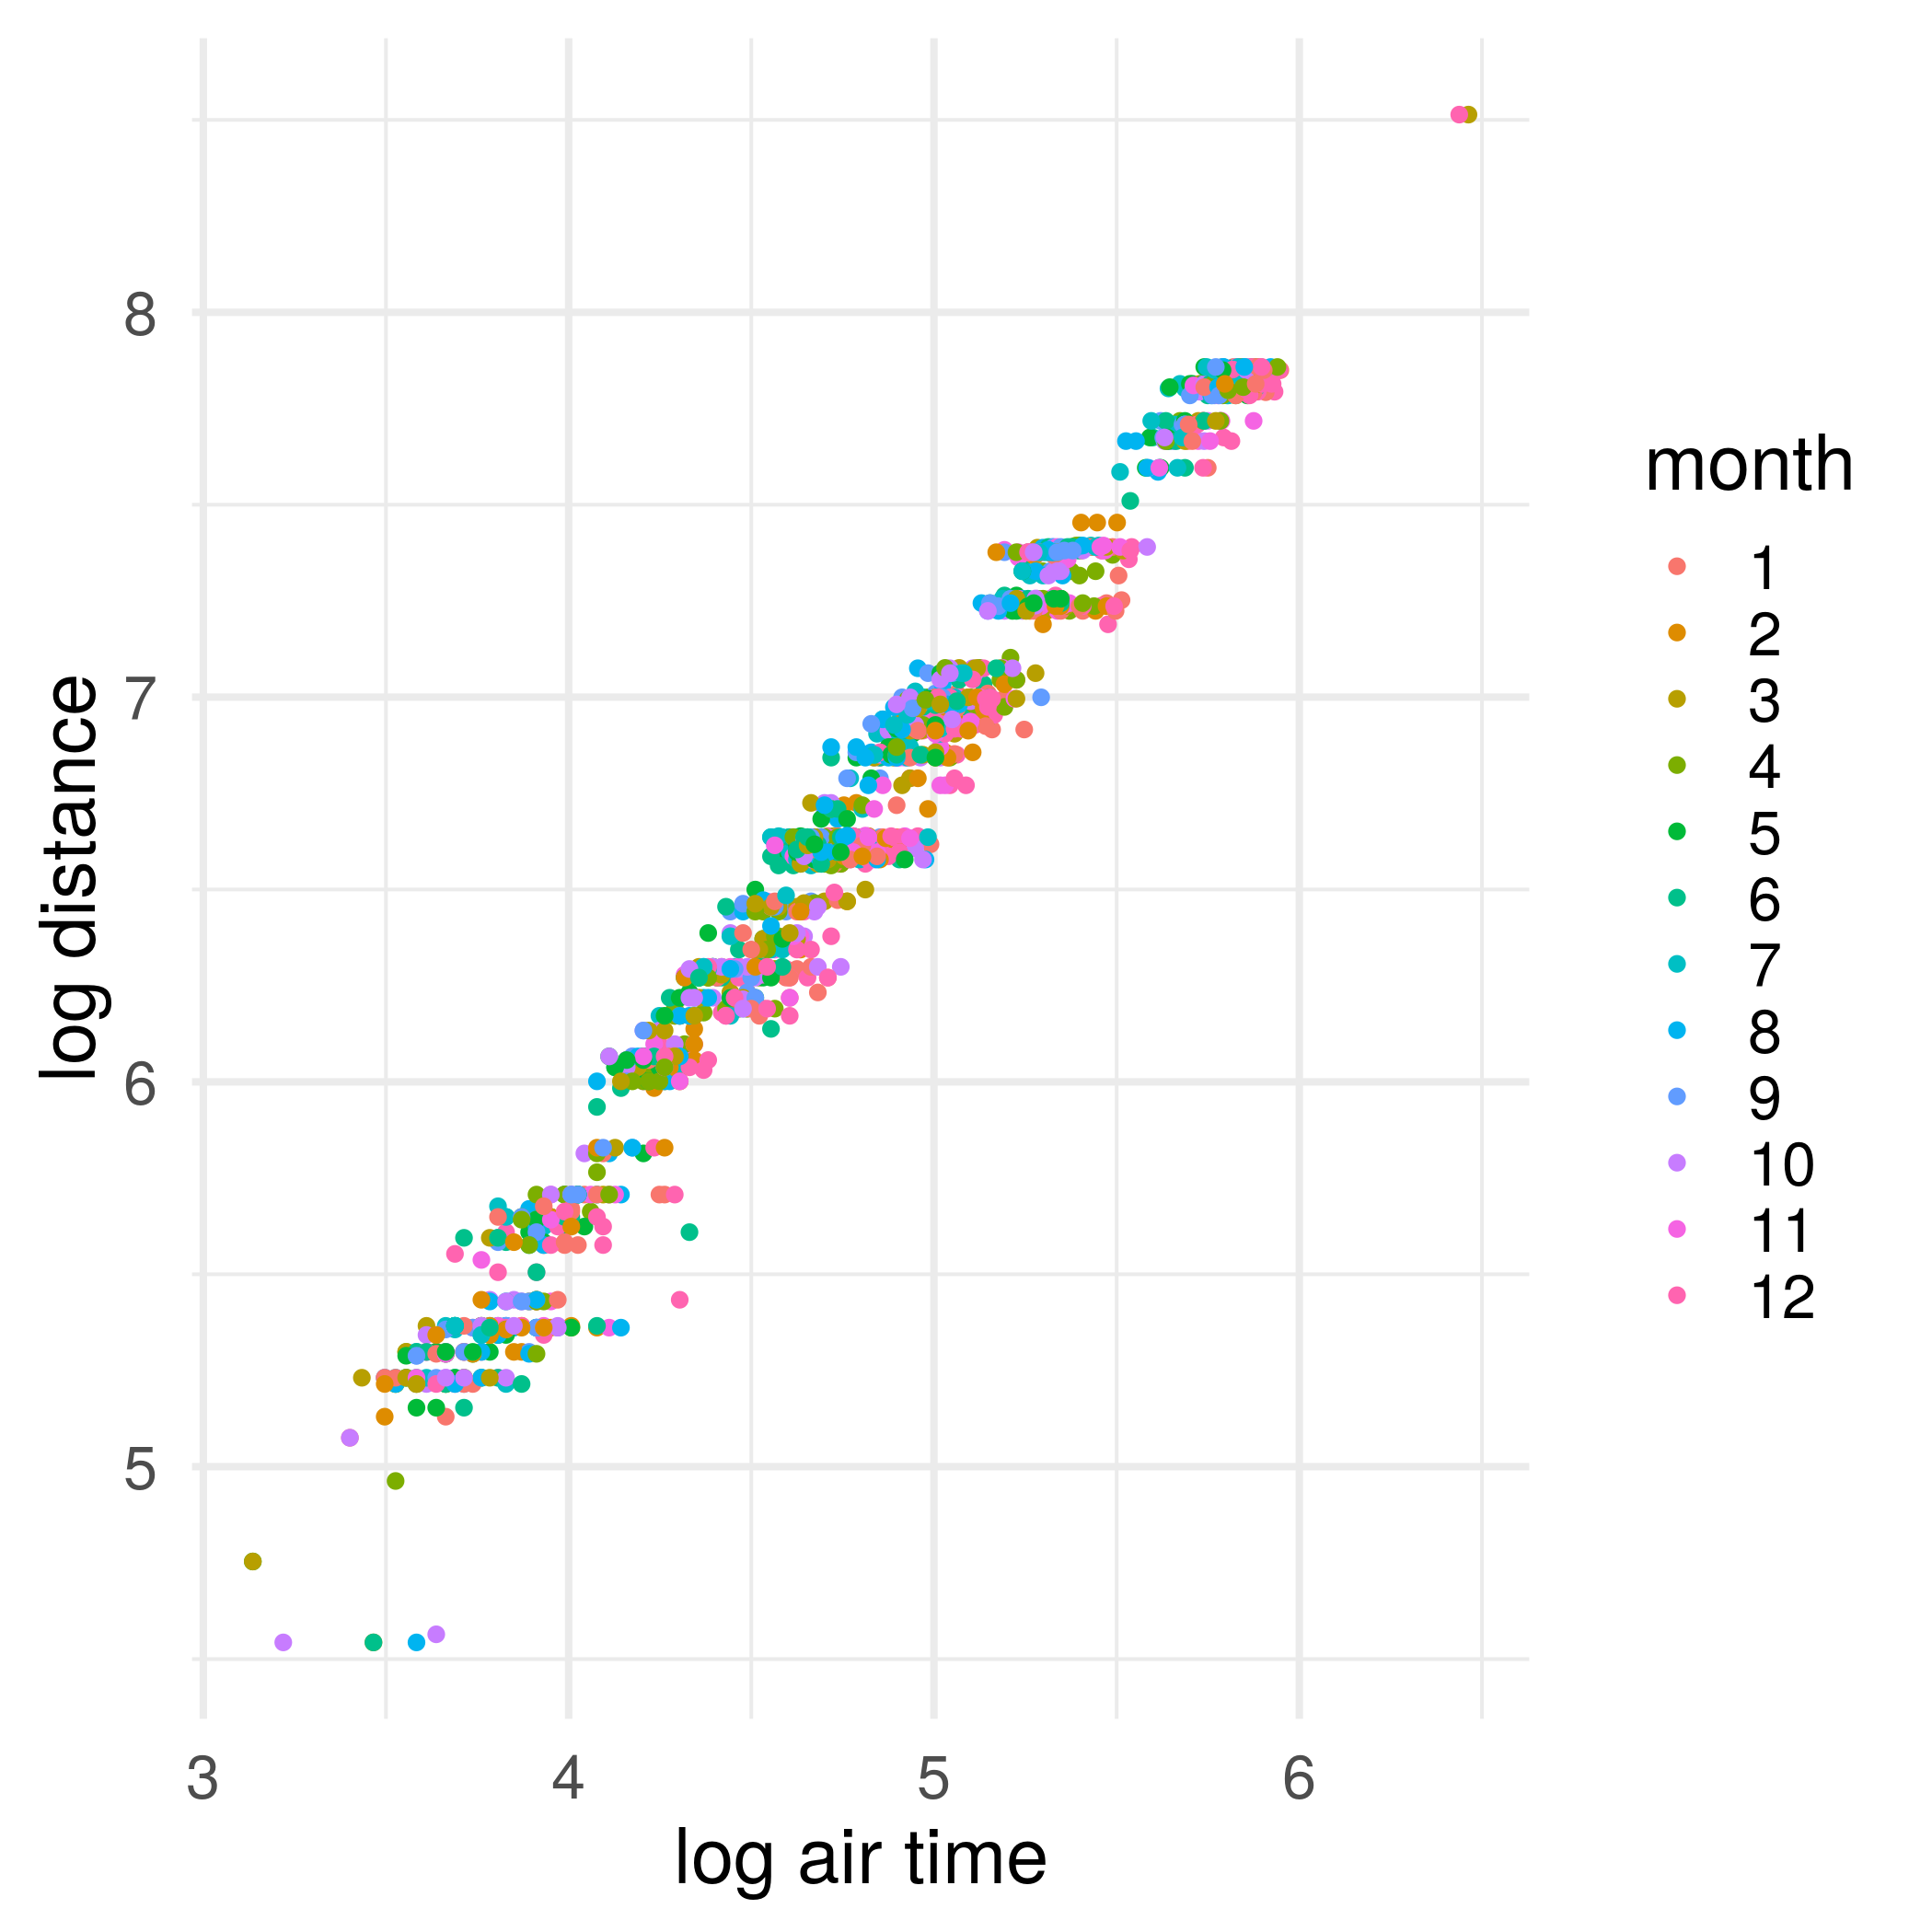
\includegraphics{figures/flight.png}
\caption{Something about flights\label{fig:flight}}
\end{figure}

\subsection{Conclusion}\label{conclusion}

Everything I know I learned from reading Fisher (1919).

\subsection*{References}\label{references}
\addcontentsline{toc}{subsection}{References}

\hypertarget{refs}{}
\hypertarget{ref-fisher1919xv}{}
Fisher, R.A. (1919). XV.---The correlation between relatives on the
supposition of mendelian inheritance. Earth and Environmental Science
Transactions of the Royal Society of Edinburgh \emph{52}, 399--433.

\end{document}
